\documentclass[11pt]{article}
\usepackage[margin=2.5cm]{geometry}
\usepackage[T1]{fontenc}
\usepackage{lmodern}
\usepackage{amsmath,amssymb,amsthm}
\usepackage{booktabs}
\usepackage{graphicx}
\usepackage[numbers,sort&compress]{natbib}
\usepackage{xcolor}
\usepackage{tikz}
\usetikzlibrary{positioning,arrows.meta,calc}
\usepackage{xurl}
\usepackage[hidelinks]{hyperref}
\usepackage{cleveref}
\usepackage{microtype}
\emergencystretch=2em
% generated by scripts/manuscript_from_report.py from the certified report -- do not edit
\newcommand{\NUsers}{200}
\newcommand{\NPairs}{2{,}000}
\newcommand{\UsersPerQ}{50}
\newcommand{\TimeLimit}{20}
\newcommand{\CertLimit}{60}
\newcommand{\EnumMax}{14}
\newcommand{\ThreatInit}{40}
\newcommand{\BeamWidth}{5}
\newcommand{\BeamDepth}{15}
\newcommand{\HeurDepth}{15}
\newcommand{\NBoot}{2{,}000}
\newcommand{\Eps}{10^{-6}}
\newcommand{\MLDataUsers}{5{,}646}
\newcommand{\MLDataItems}{1{,}979}
\newcommand{\MLKGRel}{11}
\newcommand{\MLItemsKG}{1{,}979}
\newcommand{\MLThetaCo}{31.79}
\newcommand{\MLBeta}{0.00}
\newcommand{\MLRecPop}{20.7}
\newcommand{\MLNdcgPop}{17.6}
\newcommand{\MLRecItemKNN}{28.2}
\newcommand{\MLNdcgItemKNN}{25.8}
\newcommand{\MLRecBPR}{26.7}
\newcommand{\MLNdcgBPR}{22.8}
\newcommand{\MLRecKG}{21.8}
\newcommand{\MLNdcgKG}{19.6}
\newcommand{\MLRecFull}{29.1}
\newcommand{\MLNdcgFull}{26.5}
\newcommand{\MLScope}{100.0}
\newcommand{\MLEvFree}{0}
\newcommand{\MLScopeN}{2000}
\newcommand{\LFDataUsers}{1{,}716}
\newcommand{\LFDataItems}{1{,}286}
\newcommand{\LFKGRel}{8}
\newcommand{\LFItemsKG}{1{,}010}
\newcommand{\LFThetaCo}{42.78}
\newcommand{\LFBeta}{0.48}
\newcommand{\LFRecPop}{22.0}
\newcommand{\LFNdcgPop}{10.5}
\newcommand{\LFRecItemKNN}{39.5}
\newcommand{\LFNdcgItemKNN}{23.3}
\newcommand{\LFRecBPR}{31.5}
\newcommand{\LFNdcgBPR}{17.8}
\newcommand{\LFRecKG}{22.4}
\newcommand{\LFNdcgKG}{11.8}
\newcommand{\LFRecFull}{42.2}
\newcommand{\LFNdcgFull}{25.3}
\newcommand{\LFScope}{70.3}
\newcommand{\LFEvFree}{0}
\newcommand{\LFScopeN}{2000}
\newcommand{\LFAOpt}{95.70}
\newcommand{\LFAFeas}{0.00}
\newcommand{\LFAInf}{4.30}
\newcommand{\LFATout}{0.00}
\newcommand{\LFAExists}{95.70}
\newcommand{\LFAExistsLo}{94.75}
\newcommand{\LFAExistsHi}{96.60}
\newcommand{\LFATime}{0.14}
\newcommand{\LFATimeMax}{1.00}
\newcommand{\LFAKilled}{0}
\newcommand{\LFAThreeOpt}{82.85}
\newcommand{\LFAThreeFeas}{0.00}
\newcommand{\LFAThreeInf}{17.15}
\newcommand{\LFAThreeTout}{0.00}
\newcommand{\LFAThreeExists}{82.85}
\newcommand{\LFAThreeExistsLo}{80.80}
\newcommand{\LFAThreeExistsHi}{84.75}
\newcommand{\LFAThreeTime}{0.13}
\newcommand{\LFAThreeTimeMax}{0.95}
\newcommand{\LFAThreeKilled}{0}
\newcommand{\LFBOpt}{30.05}
\newcommand{\LFBFeas}{0.00}
\newcommand{\LFBInf}{69.95}
\newcommand{\LFBTout}{0.00}
\newcommand{\LFBExists}{30.05}
\newcommand{\LFBExistsLo}{28.05}
\newcommand{\LFBExistsHi}{31.90}
\newcommand{\LFBTime}{0.02}
\newcommand{\LFBTimeMax}{0.33}
\newcommand{\LFBKilled}{0}
\newcommand{\LFCOpt}{28.05}
\newcommand{\LFCFeas}{0.00}
\newcommand{\LFCInf}{71.95}
\newcommand{\LFCTout}{0.00}
\newcommand{\LFCExists}{28.05}
\newcommand{\LFCExistsLo}{26.15}
\newcommand{\LFCExistsHi}{30.00}
\newcommand{\LFCTime}{0.02}
\newcommand{\LFCTimeMax}{0.40}
\newcommand{\LFCKilled}{0}
\newcommand{\MLAOpt}{95.30}
\newcommand{\MLAFeas}{4.70}
\newcommand{\MLAInf}{0.00}
\newcommand{\MLATout}{0.00}
\newcommand{\MLAExists}{100.00}
\newcommand{\MLAExistsLo}{100.00}
\newcommand{\MLAExistsHi}{100.00}
\newcommand{\MLATime}{2.10}
\newcommand{\MLATimeMax}{24.53}
\newcommand{\MLAKilled}{0}
\newcommand{\MLAThreeOpt}{83.85}
\newcommand{\MLAThreeFeas}{0.75}
\newcommand{\MLAThreeInf}{15.40}
\newcommand{\MLAThreeTout}{0.00}
\newcommand{\MLAThreeExists}{84.60}
\newcommand{\MLAThreeExistsLo}{82.29}
\newcommand{\MLAThreeExistsHi}{86.74}
\newcommand{\MLAThreeTime}{0.77}
\newcommand{\MLAThreeTimeMax}{23.54}
\newcommand{\MLAThreeKilled}{0}
\newcommand{\MLBOpt}{80.35}
\newcommand{\MLBFeas}{2.95}
\newcommand{\MLBInf}{16.55}
\newcommand{\MLBTout}{0.15}
\newcommand{\MLBExists}{83.30}
\newcommand{\MLBExistsLo}{80.92}
\newcommand{\MLBExistsHi}{85.75}
\newcommand{\MLBTime}{0.97}
\newcommand{\MLBTimeMax}{24.32}
\newcommand{\MLBKilled}{0}
\newcommand{\MLCOpt}{71.20}
\newcommand{\MLCFeas}{1.90}
\newcommand{\MLCInf}{26.90}
\newcommand{\MLCTout}{0.00}
\newcommand{\MLCExists}{73.10}
\newcommand{\MLCExistsLo}{70.11}
\newcommand{\MLCExistsHi}{76.05}
\newcommand{\MLCTime}{0.80}
\newcommand{\MLCTimeMax}{24.39}
\newcommand{\MLCKilled}{0}
\newcommand{\LFBAN}{601}
\newcommand{\LFBAUsers}{182}
\newcommand{\LFBAMean}{0.271}
\newcommand{\LFBALo}{0.212}
\newcommand{\LFBAHi}{0.334}
\newcommand{\LFBAMed}{0}
\newcommand{\LFBAPos}{20.0}
\newcommand{\LFBANeg}{0}
\newcommand{\LFCBN}{561}
\newcommand{\LFCBUsers}{176}
\newcommand{\LFCBMean}{0.007}
\newcommand{\LFCBLo}{0.002}
\newcommand{\LFCBHi}{0.014}
\newcommand{\LFCBMed}{0}
\newcommand{\LFCBPos}{0.7}
\newcommand{\LFCBNeg}{0}
\newcommand{\LFAThreeAN}{1657}
\newcommand{\LFAThreeAUsers}{200}
\newcommand{\LFAThreeAMean}{0.020}
\newcommand{\LFAThreeALo}{0.012}
\newcommand{\LFAThreeAHi}{0.029}
\newcommand{\LFAThreeAMed}{0}
\newcommand{\LFAThreeAPos}{1.8}
\newcommand{\LFAThreeANeg}{0}
\newcommand{\LFCAThreeN}{561}
\newcommand{\LFCAThreeUsers}{176}
\newcommand{\LFCAThreeMean}{0.246}
\newcommand{\LFCAThreeLo}{0.188}
\newcommand{\LFCAThreeHi}{0.308}
\newcommand{\LFCAThreeMed}{0}
\newcommand{\LFCAThreePos}{19.1}
\newcommand{\LFCAThreeNeg}{0}
\newcommand{\MLBAN}{1535}
\newcommand{\MLBAUsers}{198}
\newcommand{\MLBAMean}{1.348}
\newcommand{\MLBALo}{1.185}
\newcommand{\MLBAHi}{1.524}
\newcommand{\MLBAMed}{0}
\newcommand{\MLBAPos}{33.7}
\newcommand{\MLBANeg}{0}
\newcommand{\MLCBN}{1401}
\newcommand{\MLCBUsers}{198}
\newcommand{\MLCBMean}{0.313}
\newcommand{\MLCBLo}{0.250}
\newcommand{\MLCBHi}{0.377}
\newcommand{\MLCBMed}{0}
\newcommand{\MLCBPos}{15.1}
\newcommand{\MLCBNeg}{0}
\newcommand{\MLAThreeAN}{1598}
\newcommand{\MLAThreeAUsers}{200}
\newcommand{\MLAThreeAMean}{0.397}
\newcommand{\MLAThreeALo}{0.325}
\newcommand{\MLAThreeAHi}{0.479}
\newcommand{\MLAThreeAMed}{0}
\newcommand{\MLAThreeAPos}{18.9}
\newcommand{\MLAThreeANeg}{0}
\newcommand{\MLCAThreeN}{1411}
\newcommand{\MLCAThreeUsers}{199}
\newcommand{\MLCAThreeMean}{1.332}
\newcommand{\MLCAThreeLo}{1.106}
\newcommand{\MLCAThreeHi}{1.581}
\newcommand{\MLCAThreeMed}{0}
\newcommand{\MLCAThreePos}{29.4}
\newcommand{\MLCAThreeNeg}{0}
\newcommand{\LFAROne}{79.5}
\newcommand{\LFARTen}{100.0}
\newcommand{\LFAThreeROne}{50.0}
\newcommand{\LFAThreeRTen}{97.5}
\newcommand{\LFBROne}{2.5}
\newcommand{\LFBRTen}{63.5}
\newcommand{\LFCROne}{1.5}
\newcommand{\LFCRTen}{60.5}
\newcommand{\MLAROne}{100.0}
\newcommand{\MLARTen}{100.0}
\newcommand{\MLAThreeROne}{55.5}
\newcommand{\MLAThreeRTen}{100.0}
\newcommand{\MLBROne}{54.0}
\newcommand{\MLBRTen}{98.5}
\newcommand{\MLCROne}{36.0}
\newcommand{\MLCRTen}{98.5}
\newcommand{\LFAQShort}{97.4}
\newcommand{\LFAQSecond}{95.8}
\newcommand{\LFAQThird}{93.8}
\newcommand{\LFAQLong}{95.8}
\newcommand{\LFAThreeQShort}{71.2}
\newcommand{\LFAThreeQSecond}{83.4}
\newcommand{\LFAThreeQThird}{85.6}
\newcommand{\LFAThreeQLong}{91.2}
\newcommand{\LFBQShort}{11.8}
\newcommand{\LFBQSecond}{27.2}
\newcommand{\LFBQThird}{36.0}
\newcommand{\LFBQLong}{45.2}
\newcommand{\LFCQShort}{9.4}
\newcommand{\LFCQSecond}{24.8}
\newcommand{\LFCQThird}{34.4}
\newcommand{\LFCQLong}{43.6}
\newcommand{\MLAQShort}{100.0}
\newcommand{\MLAQSecond}{100.0}
\newcommand{\MLAQThird}{100.0}
\newcommand{\MLAQLong}{100.0}
\newcommand{\MLAThreeQShort}{63.0}
\newcommand{\MLAThreeQSecond}{82.6}
\newcommand{\MLAThreeQThird}{93.4}
\newcommand{\MLAThreeQLong}{99.4}
\newcommand{\MLBQShort}{57.2}
\newcommand{\MLBQSecond}{82.6}
\newcommand{\MLBQThird}{93.8}
\newcommand{\MLBQLong}{99.6}
\newcommand{\MLCQShort}{42.8}
\newcommand{\MLCQSecond}{66.4}
\newcommand{\MLCQThird}{86.8}
\newcommand{\MLCQLong}{96.4}
\newcommand{\LFKendallB}{0.71}
\newcommand{\LFKendallC}{0.71}
\newcommand{\MLKendallB}{0.73}
\newcommand{\MLKendallC}{0.77}
\newcommand{\LFCbeamSucc}{28.05}
\newcommand{\LFCbeamOnOpt}{100.00}
\newcommand{\LFCbeamExact}{100.00}
\newcommand{\LFCcontinuousgumbelattributionrepairSucc}{26.30}
\newcommand{\LFCcontinuousgumbelattributionrepairOnOpt}{93.76}
\newcommand{\LFCcontinuousgumbelattributionrepairExact}{95.25}
\newcommand{\LFCcontinuoussigmoidattributionrepairSucc}{26.60}
\newcommand{\LFCcontinuoussigmoidattributionrepairOnOpt}{94.83}
\newcommand{\LFCcontinuoussigmoidattributionrepairExact}{97.18}
\newcommand{\LFCgreedylistawareSucc}{18.75}
\newcommand{\LFCgreedylistawareOnOpt}{66.84}
\newcommand{\LFCgreedylistawareExact}{93.33}
\newcommand{\LFCgreedymarginSucc}{14.35}
\newcommand{\LFCgreedymarginOnOpt}{51.16}
\newcommand{\LFCgreedymarginExact}{91.64}
\newcommand{\LFCgreedypopularitySucc}{6.45}
\newcommand{\LFCgreedypopularityOnOpt}{22.99}
\newcommand{\LFCgreedypopularityExact}{75.97}
\newcommand{\LFCgreedyrandomSucc}{8.15}
\newcommand{\LFCgreedyrandomOnOpt}{29.06}
\newcommand{\LFCgreedyrandomExact}{77.30}
\newcommand{\LFCgreedytargetscoreSucc}{12.85}
\newcommand{\LFCgreedytargetscoreOnOpt}{45.81}
\newcommand{\LFCgreedytargetscoreExact}{95.72}
\newcommand{\LFCgreedytargetscorecOneStopSucc}{11.75}
\newcommand{\LFCgreedytargetscorecOneStopOnOpt}{41.89}
\newcommand{\LFCgreedytargetscorecOneStopExact}{97.45}
\newcommand{\LFCStopCOne}{94.65}
\newcommand{\LFCStopList}{13.0}
\newcommand{\LFCStopAll}{12.4}
\newcommand{\LFCgreedyviolationSucc}{27.15}
\newcommand{\LFCgreedyviolationOnOpt}{96.79}
\newcommand{\LFCgreedyviolationExact}{98.89}
\newcommand{\MLCbeamSucc}{63.45}
\newcommand{\MLCbeamOnOpt}{87.43}
\newcommand{\MLCbeamExact}{95.90}
\newcommand{\MLCcontinuousgumbelattributionrepairSucc}{71.35}
\newcommand{\MLCcontinuousgumbelattributionrepairOnOpt}{97.54}
\newcommand{\MLCcontinuousgumbelattributionrepairExact}{63.50}
\newcommand{\MLCcontinuoussigmoidattributionrepairSucc}{71.30}
\newcommand{\MLCcontinuoussigmoidattributionrepairOnOpt}{97.47}
\newcommand{\MLCcontinuoussigmoidattributionrepairExact}{68.52}
\newcommand{\MLCgreedylistawareSucc}{44.20}
\newcommand{\MLCgreedylistawareOnOpt}{61.10}
\newcommand{\MLCgreedylistawareExact}{72.18}
\newcommand{\MLCgreedymarginSucc}{45.40}
\newcommand{\MLCgreedymarginOnOpt}{62.50}
\newcommand{\MLCgreedymarginExact}{75.96}
\newcommand{\MLCgreedypopularitySucc}{15.10}
\newcommand{\MLCgreedypopularityOnOpt}{20.93}
\newcommand{\MLCgreedypopularityExact}{37.25}
\newcommand{\MLCgreedyrandomSucc}{15.10}
\newcommand{\MLCgreedyrandomOnOpt}{21.21}
\newcommand{\MLCgreedyrandomExact}{26.49}
\newcommand{\MLCgreedytargetscoreSucc}{32.10}
\newcommand{\MLCgreedytargetscoreOnOpt}{44.52}
\newcommand{\MLCgreedytargetscoreExact}{63.56}
\newcommand{\MLCgreedytargetscorecOneStopSucc}{21.80}
\newcommand{\MLCgreedytargetscorecOneStopOnOpt}{30.06}
\newcommand{\MLCgreedytargetscorecOneStopExact}{76.17}
\newcommand{\MLCStopCOne}{79.15}
\newcommand{\MLCStopList}{35.8}
\newcommand{\MLCStopAll}{27.5}
\newcommand{\MLCgreedyviolationSucc}{62.05}
\newcommand{\MLCgreedyviolationOnOpt}{85.53}
\newcommand{\MLCgreedyviolationExact}{90.72}
\newcommand{\AlphaExistsLow}{79.8}
\newcommand{\AlphaExistsHalf}{76.2}
\newcommand{\AlphaExistsHigh}{72.9}
\newcommand{\AlphaExistsOne}{69.9}
\newcommand{\KFiveAExists}{100.00}
\newcommand{\KFiveATout}{0.00}
\newcommand{\KFiveBExists}{93.20}
\newcommand{\KFiveBTout}{0.00}
\newcommand{\KFiveCExists}{88.00}
\newcommand{\KFiveCTout}{0.00}
\newcommand{\KTenAExists}{100.00}
\newcommand{\KTenATout}{0.00}
\newcommand{\KTenBExists}{84.70}
\newcommand{\KTenBTout}{0.20}
\newcommand{\KTenCExists}{74.90}
\newcommand{\KTenCTout}{0.10}
\newcommand{\KTwentyAExists}{100.00}
\newcommand{\KTwentyATout}{0.00}
\newcommand{\KTwentyBExists}{70.95}
\newcommand{\KTwentyBTout}{1.75}
\newcommand{\KTwentyCExists}{54.70}
\newcommand{\KTwentyCTout}{0.00}
\newcommand{\EnumPairs}{190}
\newcommand{\EnumUsers}{19}
\newcommand{\EnumAgree}{190}
\newcommand{\MLCertConfirmed}{7790}
\newcommand{\MLCertCorrected}{1}
\newcommand{\MLCertUndecided}{28}
\newcommand{\MLCertNotApplicable}{181}
\newcommand{\LFCertConfirmed}{8000}
\newcommand{\LFCertCorrected}{0}
\newcommand{\LFCertUndecided}{0}
\newcommand{\LFCertNotApplicable}{0}
\newcommand{\LFCauseEv}{0.4}
\newcommand{\LFCauseJoint}{2.4}
\newcommand{\LFCauseList}{91.2}
\newcommand{\MLCauseEv}{18.2}
\newcommand{\MLCauseJoint}{19.9}
\newcommand{\MLCauseList}{61.5}
\newcommand{\SmallerThanOpt}{0}
\newcommand{\SuccessOnInf}{0}


\newtheorem{definition}{Definition}
\newtheorem{proposition}{Proposition}
\newcommand{\topk}{\operatorname{top}\text{-}K}
\newcommand{\Peps}{P_\varepsilon}

\title{EPIC-Rec: Evidence-Preserving Counterfactual Explanations\\for Top-$K$ Graph Recommendation}
\author{Mehrdad Jalali\\
\small Department of Applied Data Science and Artificial Intelligence\\
\small School of Arts, Information and Media, SRH University of Applied Sciences Heidelberg, Germany
\and
Majid Vafaei Jahan\\
\small Department of Computer Engineering, Ma.C., Islamic Azad University, Mashhad, Iran}
\date{}

\begin{document}
\maketitle

\begin{abstract}
Counterfactual explanations for recommender systems name a small set of past interactions whose removal changes a
recommendation. Existing methods remove the target item but leave the rest of the list to chance, and they do not ask
whether the reasons behind the remaining recommendations survive the edit. We study the stricter question: can one
recommendation be removed with a minimal edit to the user's history while every other top-$K$ item stays in the list
and keeps at least one of its original, score-contributing evidence paths? We formulate this as a constrained
minimum-mask problem with three conditions---removal (C1), membership preservation (C2) and evidence preservation
(C3)---and introduce EPIC-Rec (Evidence-Preserving Interaction Counterfactuals for Recommendation). On an inductive, additive path-scoring recommender the problem becomes a mixed-integer linear program that we solve
for a margin variant, using lazy constraint generation. Every optimality or infeasibility claim is
re-checked under a second configuration of the same solver, HiGHS. That cross-check is not a formal certificate. On MovieLens-1M, across \NPairs{} user--target pairs from \NUsers{}
users, a mask that removes the target exists for \MLAExists\% of pairs, a mask that also keeps the other $K-1$ items
for \MLBExists\% [\MLBExistsLo, \MLBExistsHi], and one that also keeps their evidence for \MLCExists\% [\MLCExistsLo,
\MLCExistsHi]. On Last.fm the same three rates are \LFAExists\% [\LFAExistsLo, \LFAExistsHi], \LFBExists\%
[\LFBExistsLo, \LFBExistsHi] and \LFCExists\% [\LFCExistsLo, \LFCExistsHi]. A target-score order that stops at
removal keeps the list and the evidence in only \MLCStopAll\% of the MovieLens edits that do remove the target, and
in \LFCStopAll\% of such Last.fm edits. Those two rates are conditional on removal. On all \NPairs{} pairs the same
MovieLens edits satisfy C1 + C2 + C3 for \MLCgreedytargetscorecOneStopSucc\%. Surgical counterfactuals are common on
MovieLens and uncommon on Last.fm. The Last.fm gap appears already when the list must be kept, before evidence is
required.
\end{abstract}

\section{Introduction}

Counterfactual explanations justify an individual algorithmic decision by naming a small change to the input that
would have produced a different output~\cite{wachter2017counterfactual}. In recommendation, the input a user controls
is their interaction history, and an explanation takes the form ``had you not watched X and Y, you would not have been
recommended Z''~\cite{ghazimatin2020prince,tran2021accent}. Recent work has extended such explanations to graph-based
recommenders~\cite{chen2022grease,chen2025grease,medda2024gnnuers}, to learned and attribution-based
explainers~\cite{barkan2024lxr,gurevitch2025lxr,barkan2026spinrec}, to sequential models~\cite{kim2026trace}, and to
evaluation protocols that look beyond the top-1 item~\cite{nguyen2026cfexprec,mohammadi2025beyond}. The closest work,
CoSRec~\cite{zhang2026cosrec}, learns sparse interaction masks for a fixed graph recommender, verifies them by
recomputing the ranking, and reports how much of the surrounding list remains stable.

What these methods do not provide is a \emph{guarantee} about the rest of the list. A mask that removes the target may
also push other items out, and it may destroy the evidence that justified them. Stability is measured after the fact,
not enforced. For a user who wants one unwanted recommendation gone, or for an auditor who wants to know whether a
recommendation can be explained independently of its neighbours, the relevant question is stricter:

\begin{quote}
\emph{Can we remove a specific recommendation with a minimal edit to the user's history while preserving every other
top-$K$ item and at least one of its original, score-contributing evidence paths?}
\end{quote}

Why would one recommendation need to be removed without disturbing the others? Three situations motivate the
question. First, user control: a user who presses ``not interested'' on one item---a title watched for a child, a
one-off gift purchase, a product already bought elsewhere---expects that item to disappear, not the rest of a list
they were satisfied with. Second, privacy: a single recommendation can reveal a sensitive inference about the user,
and removing it should not degrade unrelated suggestions. Third, explanation and audit: even when nothing is actually
removed, a minimal counterfactual (``had you not interacted with A and C, T would not have been recommended'') is a
verifiable account of why an item was recommended, and transparency obligations for recommender systems, such as
those in the EU Digital Services Act~\cite{dsa2022}, ask platforms to explain the main parameters of their
recommendations and to offer users control over them. When surgical removal is impossible, that fact is itself
informative: it shows that the recommendation is entangled with others in the list and cannot be explained or
withdrawn in isolation.

We make four contributions.
\begin{enumerate}
  \item A problem formulation with a joint guarantee: target removal (C1), exact top-$K$ membership preservation for
  the other $K-1$ items (C2), and survival of at least one original, score-contributing evidence path for each of
  them (C3), with an explicit ranking rule and an explicit evidence unit (\Cref{sec:problem}).
  \item An exact solution method. On an inductive, additive path scorer every score is linear in the binary mask,
  and a margin version of the problem becomes a mixed-integer linear program (MILP) that we solve with lazy
  constraint generation; C3 reduces to covering constraints (\Cref{sec:method}). We measure how often the margin
  version and the original problem differ.
  \item A measured cost of each constraint on MovieLens-1M and Last.fm: how many user--target pairs admit a
  mask, how many are proven infeasible, and the paired increase in minimum mask size from C1 to C1 + C2 to
  C1 + C2 + C3, stratified by target rank and history length (\Cref{sec:results}).
  \item Evidence that constraint-unaware heuristics rarely satisfy C2 and C3 by chance, and a comparison of
  heuristics and beam search with the exact optimum.
\end{enumerate}

The counterfactual edge-mask mechanism builds on our earlier work on counterfactual inverse link prediction
(CILP)~\cite{jalali2026cilp}, which removes edges from unipartite social graphs. EPIC-Rec moves this idea to
user--item--entity graphs, replaces a single link prediction with a ranked list, and adds the evidence constraint.
\Cref{fig:overview} illustrates the problem and the method.

\begin{figure}[!tbp]
\centering
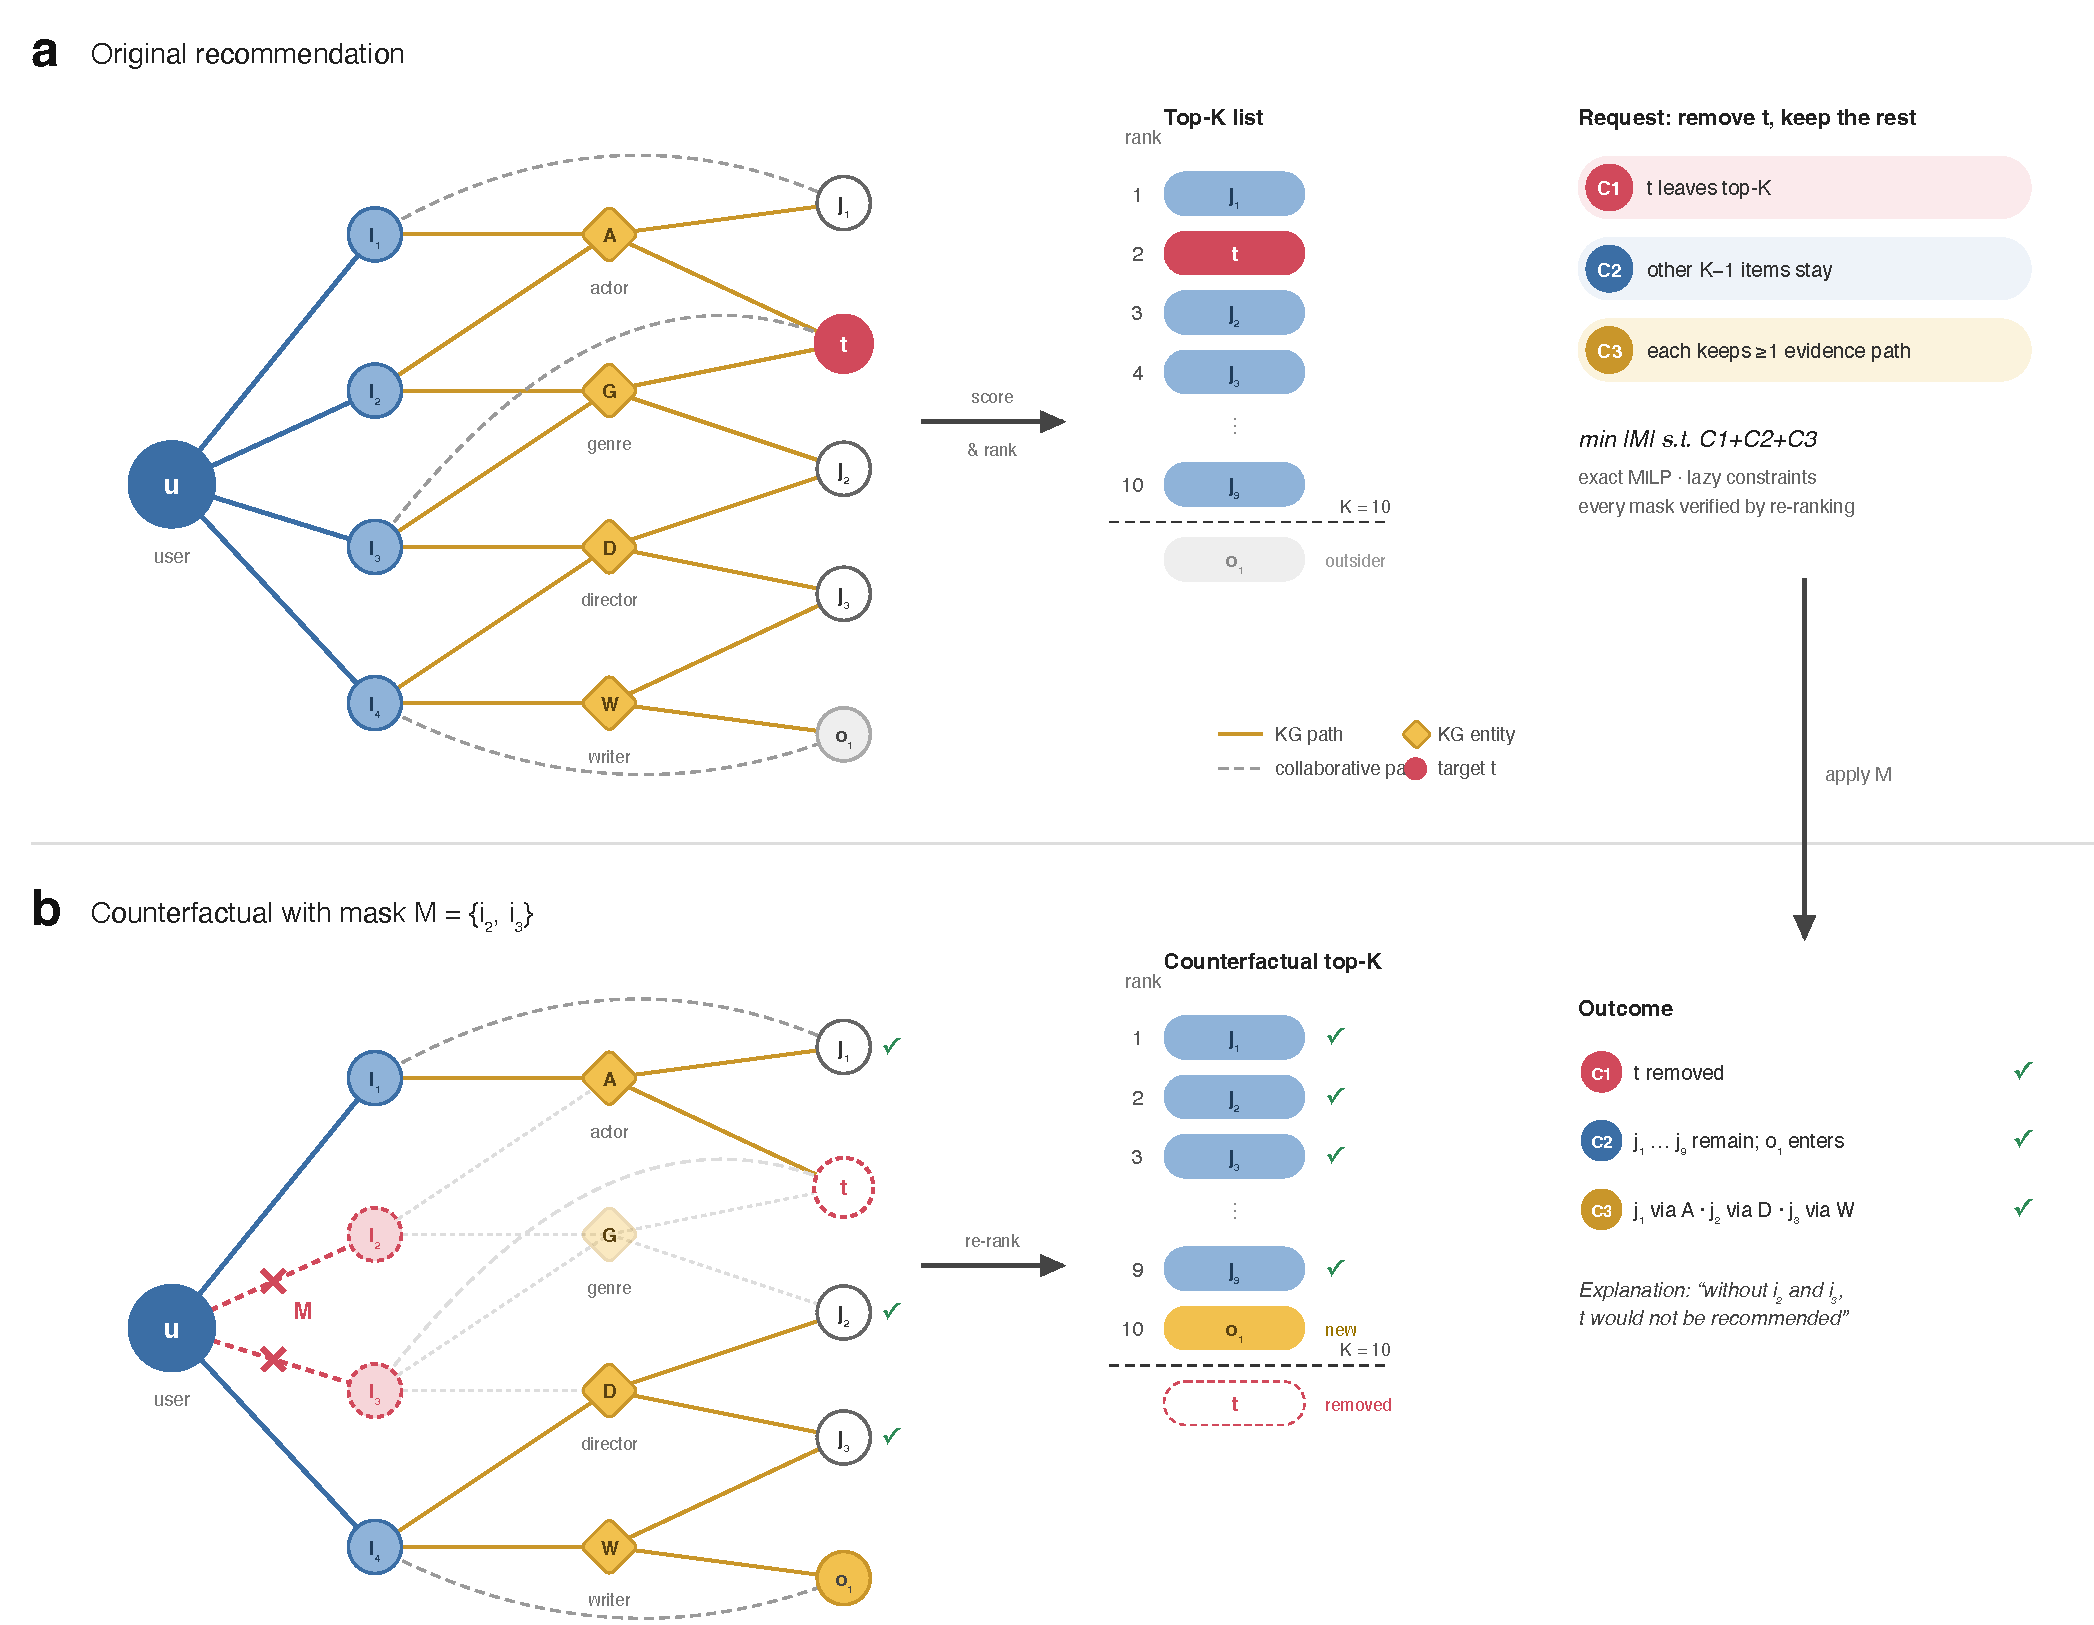
\includegraphics[width=0.92\linewidth]{fig1_epic_rec.pdf}
\caption{\textbf{EPIC-Rec removes one recommendation while keeping the rest of the top-$K$ list and its evidence.}
\textbf{a}, User $u$'s history ($i_1$--$i_4$) reaches candidate items through knowledge-graph entities (diamonds;
solid lines) and collaborative paths (dashed). Scores are sums of path contributions, giving a top-$K$ list ($K=10$)
that contains the target $t$; $o_1$ is the best item outside the list. EPIC-Rec looks for the smallest set of history
interactions $M$ to mask such that $t$ leaves the list (C1), the other $K-1$ items stay (C2), and each keeps at least
one of its original evidence paths (C3). The problem is solved as a mixed-integer linear program for the margin
problem $P_\varepsilon$ on the permitted interactions $D_u(t)$, and every returned mask is checked by re-ranking.
\textbf{b}, Masking $M=\{i_2,i_3\}$ removes their paths (faded). $t$ leaves the list, $j_1$--$j_9$ remain, each
supported by a surviving path ($\checkmark$), and $o_1$ takes the free slot. The measured rates are in
\Cref{fig:charts}.}
\label{fig:overview}
\end{figure}

\begin{figure}[!tbp]
\centering
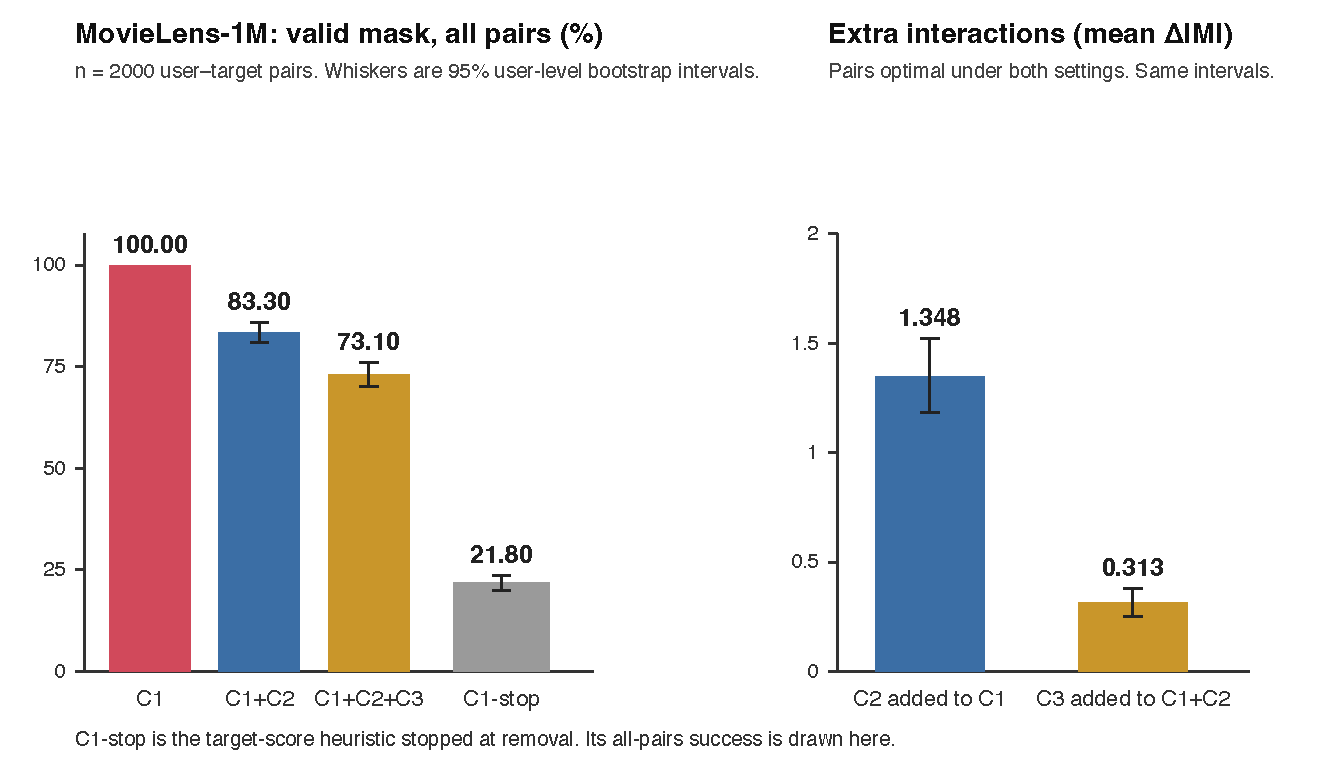
\includegraphics[width=\linewidth]{fig1_charts.pdf}
\caption{\textbf{MovieLens-1M rates on one denominator.} Both panels use all \NPairs{} pairs.
Left: a mask exists for \MLAExists\%, \MLBExists\% and \MLCExists\% of pairs under C1, C1 + C2 and
C1 + C2 + C3. The grey bar is the target-score heuristic that stops at removal and, on those same pairs,
happens to satisfy C1 + C2 + C3 (\MLCgreedytargetscorecOneStopSucc\%). Among only the edits that do remove the
target, that share is \MLCStopAll\%; that conditional rate is not drawn.
Right: paired increase in minimum mask size when C2 is added to C1 (\MLBAMean{} [\MLBALo, \MLBAHi]) and when C3
is then added (\MLCBMean{} [\MLCBLo, \MLCBHi]). Whiskers are 95\% user-level bootstrap intervals. Last.fm is in
\Cref{tab:status}.}
\label{fig:charts}
\end{figure}

\section{Related work}
\label{sec:related}

\paragraph{History-based counterfactual explainers.} PRINCE~\cite{ghazimatin2020prince} finds minimal sets of user
actions that replace the top recommendation of a personalised-PageRank recommender over a heterogeneous graph.
We do not run PRINCE at the scale of this study: it explains that recommender rather than the path-additive backbone,
and no comparison under C2 or C3 is claimed.
ACCENT~\cite{tran2021accent} extends influence functions to pairs of items and removes the user's most influential
interactions until the top recommendation is replaced. LXR~\cite{barkan2024lxr,gurevitch2025lxr} trains an explainer
network with counterfactual loss terms that scores the relevance of each piece of user data to a recommended item;
the journal version adds per-explanation fine-tuning at inference time. SPINRec~\cite{barkan2026spinrec} computes
path-integrated attributions for implicit-feedback data, sampling several plausible user profiles as baselines and
keeping the most faithful integration path. These methods explain one recommended item; they do not constrain the
rest of the list.

\paragraph{Graph explainers for recommendation.} GREASE~\cite{chen2022grease} trains a surrogate GNN around the
user--item pair and optimises perturbations of its adjacency matrix to obtain factual and counterfactual explanations;
it has been extended to top-$k$ recommendation~\cite{chen2025grease}. GNNUERS~\cite{medda2024gnnuers} perturbs the
user--item graph to explain unfairness, and CF-GNNExplainer~\cite{lucic2022cfgnn} removes edges to flip node
predictions. CoSRec~\cite{zhang2026cosrec} learns a sparse retention mask over a user's interactions for a frozen
LightGCN~\cite{he2020lightgcn} with a ranking loss and a sparsity penalty, verifies the change by recomputation, and
measures list stability. EPIC-Rec differs by enforcing membership as a hard constraint and by requiring evidence to
survive.

\paragraph{Path-based explanations.} Semantic knowledge has long been used to enrich usage-based
recommendation~\cite{abrishami2012semantic}, and knowledge-graph recommenders such as KGAT~\cite{wang2019kgat} and
RippleNet~\cite{wang2018ripplenet} propagate preferences along entity paths. CERec~\cite{wang2024cerec} uses
reinforced path reasoning to generate attribute-level counterfactuals over a knowledge graph,
PEARLM~\cite{balloccu2023pearlm} constrains path generation to paths that exist in the graph, and
CountER~\cite{tan2021counter} perturbs item aspects. None of them asks whether the paths that justify \emph{other}
recommendations survive a counterfactual edit.

\paragraph{Sequential and list-level evaluation.} TRACE~\cite{kim2026trace} produces training-free, ranking-aware
bring-in and push-out counterfactuals for sequential recommenders from score queries.
CFExpRec~\cite{nguyen2026cfexprec} and Beyond Top-1~\cite{mohammadi2025beyond,mohammadi2026beyond} show that
evaluating explanations at top-1 gives inconsistent conclusions and propose top-$K$ protocols. We follow this
list-level view, but as a constraint on the explanation rather than only as an evaluation metric.

\section{Problem formulation}
\label{sec:problem}

\paragraph{Setting and ranking rule.} User $u$ has training history $H_u$. A fixed recommender scores every item of
the candidate pool $C_u$, the catalogue minus $H_u$. For a mask $M\subseteq H_u$ let $s_M(j)$ be the score of $j$
computed from $H_u\setminus M$. Items of $C_u$ are ranked by $s_M$ in descending order, \emph{ties broken by item
identifier in ascending order}; $\topk(M)$ is the first $K$ items of this order. This one rule is used by the
recommender, by the verifier and by every search method. $L_u=\topk(\emptyset)$ is the original list, $t\in L_u$ the
target, $R=L_u\setminus\{t\}$ the retained items and $O=C_u\setminus L_u$ the outsiders.

\paragraph{Mask domain.} The mask is restricted to $D_u(t)=\{i\in H_u: A_{it}>0\}$, the interactions with at least
one path to $t$ (\Cref{sec:method}), so that an explanation names only interactions that support the target. On
MovieLens-1M this restriction removes nothing: $D_u(t)$ covers \MLScope\% of the history, because collaborative
paths connect every scored pair. On Last.fm it covers \LFScope\%.

\paragraph{Evidence unit: the individual path.} The unit of evidence is one path $p=(i,\rho,x,j)$ from an
interaction $i\in H_u$ through relation $\rho$ and intermediate node $x$ to item $j$. For a knowledge-graph relation,
$x$ is an entity that $i$ and $j$ share through $\rho$ ($i\xrightarrow{\rho}x\xleftarrow{\rho}j$); for the
collaborative relation, $x$ is another user who interacted with both $i$ and $j$ in the training data
($i\leftarrow x\to j$). The path's origin is $e(p)=i$; the path survives $M$ when $e(p)\notin M$. Its contribution
$c(p)$ is the amount it adds to $s(j)$ (\Cref{sec:method}); on our backbone it does not depend on what else is masked.
Two paths that share an origin and a relation but pass through different entities or users are different pieces of
evidence.

\begin{definition}[Original evidence set]
For a retained item $j\in R$ let $\tau_{j}=\max(\alpha\max_{p\to j}c(p),\,\phi)$, with $\alpha\in(0,1]$ and the
maximum taken over all paths from $H_u$ to $j$. The floor $\phi\ge 0$ is a minimum contribution. The original
evidence set of $j$ is $P_j=\{p\to j: c(p)\ge\tau_j\}$. This study sets $\phi=0$, so $\tau_j$ is the relative
threshold. A path of contribution 0 is never evidence.
\end{definition}

The threshold is relative to the item's strongest single path, so the same $\alpha$ is comparable across users and
items. A retained item with no path from $H_u$ has an empty evidence set and cannot satisfy C3; such items make
setting C infeasible for the pair, and we report how often this happens. On both main samples that count is
\MLEvFree{} (MovieLens) and \LFEvFree{} (Last.fm). A surviving path is accepted as evidence only if disabling that
single path lowers the recomputed score of $j$ by a positive amount and by at least $\phi$. That check is a
property of the additive score in \eqref{eq:backbone}. It is not a claim that the path caused the user to like the
item, or that a person would find the path a useful explanation.

\begin{definition}[Problem $P$]
Find $M\subseteq D_u(t)$ of minimum size such that
\begin{align*}
&\textbf{C1 (removal)} && t\notin\topk(M),\\
&\textbf{C2 (membership)} && R\subseteq\topk(M),\\
&\textbf{C3 (evidence)} && \forall j\in R\;\exists p\in P_j:\ e(p)\notin M.
\end{align*}
Setting A asks for C1 only, setting B for C1 + C2, and setting C for C1 + C2 + C3. Setting A3, used only as an
ablation, asks for C1 + C3 and drops the list constraint.
\end{definition}

Retained items may reorder, and under C1+C2 exactly one outsider takes the freed position.

\paragraph{Margin variant $\Peps$.} A MILP cannot express ``ranked above, ties broken by identifier'' without strict
inequalities, so the solver works on a margin variant in which every ordering the constraints need holds with a gap of
at least $\varepsilon=10^{-6}$ in masked score:
\begin{align*}
&\textbf{A}_\varepsilon && \bigl|\{c\in C_u\setminus\{t\}: s_M(c)\ge s_M(t)+\varepsilon\}\bigr|\ge K,\\
&\textbf{B}_\varepsilon && \exists r\in O:\ s_M(r)\ge s_M(t)+\varepsilon\ \text{and, for every } j\in R,\\
& && \qquad s_M(j)\ge s_M(t)+\varepsilon\ \text{and}\ s_M(j)\ge s_M(c)+\varepsilon\ \ \forall c\in O\setminus\{r\},\\
&\textbf{C}_\varepsilon && \textbf{B}_\varepsilon\ \text{and C3}.
\end{align*}

\begin{proposition}\label{prop:eps}
Every mask feasible for $\Peps$ is feasible for $P$ in the same setting. Hence the $\Peps$ optimum is an upper bound on
the $P$ optimum. The two problems can differ only when a mask needs an ordering with a gap in $[0,\varepsilon)$, in
particular an exact tie resolved by item identifier.
\end{proposition}
\begin{proof}[Proof sketch]
Under A$_\varepsilon$, $K$ items score strictly above $t$, so $t$ is not in the first $K$ whatever the tie rule.
Under B$_\varepsilon$, each retained item is beaten at most by other retained items and by $r$, so it ranks within the
first $K$; and $t$ is beaten by the $K-1$ retained items and by $r$. C3 does not involve the ranking.
\end{proof}

A proof of infeasibility for $\Peps$ is therefore not a proof for $P$, and a $\Peps$ optimum can exceed the $P$
optimum. Infeasibility on $D_u(t)$ is likewise not infeasibility over the whole history: interactions outside
$D_u(t)$ are not decision variables. We measure the gap between $P$ and $\Peps$ by exhaustive search on every pair
with $|D_u(t)|\le\EnumMax$ in a separate MovieLens sample (\Cref{sec:semantics}). That sample is evidence for those
pairs, not a proof that the two problems agree in general. The main samples are not enumerated.

\paragraph{Scope of strict preservation.} Related items---a sequel, a film by the same director---often share the
target's evidence, and a user may expect them to disappear too. Strict $K-1$ preservation is therefore used in two
roles: as a diagnostic that measures how entangled a recommendation is with the rest of the list, and as a
single-item filter for users who endorse the remaining items.

\section{Method}
\label{sec:method}

\subsection{An inductive, additive path backbone}

Study~1 uses a recommender whose score is an explicit sum over evidence paths:
\begin{equation}
s(u,j)=\beta\log(1+\mathrm{pop}_j)+\frac{1}{|H_u|}\sum_{i\in H_u}\sum_{\rho\in\mathcal{R}}\theta_\rho S_\rho[i,j],
\label{eq:backbone}
\end{equation}
where for a knowledge-graph relation $\rho$
$S_\rho[i,j]=\sum_{x}1/\deg_\rho(x)$ over the entities $x$ that $i$ and $j$ share through $\rho$, and for the
collaborative relation $S_{\mathrm{co}}[i,j]=\mathrm{co}(i,j)/\sqrt{\mathrm{pop}_i\,\mathrm{pop}_j}$, one term per
co-interacting user. Each summand is one path $p$ with contribution
$c(p)=\theta_\rho/(\deg_\rho(x)|H_u|)$ or $c(p)=\theta_{\mathrm{co}}/(\sqrt{\mathrm{pop}_i\mathrm{pop}_j}\,|H_u|)$;
the normalisations are frozen at their pre-mask values. Co-occurrence counts and popularity are computed on the
training split. MovieLens keeps the \MLKGRel{} Satori film relations that survive the frequency filter; Last.fm keeps
the \LFKGRel{} music relations released with KGCN~\cite{wang2019kgcn}. Collaborative and trust-based signals remain central to recommendation~\cite{faridani2017trust}; our
backbone represents the collaborative signal as explicit co-interaction paths, so it enters the evidence sets like
any knowledge-graph relation. There is no user embedding, so masking removes all of $M$'s signal and no retraining is needed. The
weights $\theta_\rho\ge0$ and $\beta\ge0$ are learned with BPR~\cite{rendle2009bpr} under non-negativity constraints
on leave-one-out features: for a training triple $(u,p,n)$ the model input is $H_u\setminus\{p\}$, and the
co-occurrence and popularity statistics that contain $u$'s own interaction with $p$ are corrected accordingly.

Two consequences make the problem tractable. Masking interaction $i$ subtracts a fixed row,
$s_M(j)=s(j)-\sum_{i\in M}A_{ij}$ with $A_{ij}=W_{ij}/|H_u|$ and $W=\sum_\rho\theta_\rho S_\rho$, so every score is
linear in the mask. And a surviving path's contribution does not depend on the mask, so with
$P_{ij}=\max_{p:\,e(p)=i,\,p\to j}c(p)$ the largest single-path contribution from $i$ to $j$, C3 holds for $j$ if and
only if some interaction in $Q_j=\{i:P_{ij}\ge\tau_j\}$ is unmasked.

\subsection{Exact MILP for \texorpdfstring{$\Peps$}{P-epsilon}}

Let $m_i\in\{0,1\}$ indicate $i\in M$ for $i\in D_u(t)$ and $z_r\in\{0,1\}$ select the replacement among a candidate
set $\mathcal{O}\subseteq O$. Writing $\Delta_{ab}(m)=s(a)-s(b)-\sum_im_i(A_{ia}-A_{ib})$, setting C is
\begin{align}
\min\ &\textstyle\sum_i m_i \nonumber\\
\text{s.t. }&\textstyle\sum_{r\in\mathcal{O}}z_r=1, \qquad \Delta_{rt}(m)\ge\varepsilon-B_{rt}(1-z_r)\ \ \forall r\in\mathcal{O},\\
&\Delta_{jt}(m)\ge\varepsilon\ \ \forall j\in R,\\
&\Delta_{jc}(m)\ge\varepsilon-B_{jc}z_c\ \ \forall j\in R,\ c\in O\ \ (z_c\equiv0\ \text{for}\ c\notin\mathcal{O}),\label{eq:threat}\\
&\textstyle\sum_{i\in Q_j\cap D_u(t)}(1-m_i)\ge1\ \ \forall j\in R \text{ with } Q_j\subseteq D_u(t).\label{eq:cover}
\end{align}
An interaction outside $D_u(t)$ has no mask variable: it is fixed unmasked. If $Q_j$ meets the complement of
$D_u(t)$, item $j$ already keeps a qualifying origin that the program cannot delete, and \eqref{eq:cover} is omitted.
Setting B drops \eqref{eq:cover}; setting A3 keeps it and drops the list constraints; setting A replaces the ordering
constraints by indicators $y_c$, one per candidate, and requires $\sum_cy_c\ge K$. Each big-$M$ constant is the
tightest valid value for its row, $B_{ab}=\max(0,\varepsilon-\min_m\Delta_{ab}(m))$. The score margin is
$\varepsilon=10^{-6}$. The study configuration sets HiGHS primal and MIP feasibility tolerances to $10^{-9}$, three
orders of magnitude smaller than $\varepsilon$. The verifier accepts a required gap down to $\varepsilon-10^{-9}$.

\paragraph{Replacement pruning.} Let $\mathrm{lb}(c)=s(c)-\sum_{i\in D_u(t)}A_{ic}$ be the lowest score $c$ can reach.
The replacement must satisfy $s(r)\ge\mathrm{lb}(t)+\varepsilon$, and we may further restrict it to
$s(r)\ge\max_{c\in O}\mathrm{lb}(c)$. The reason: if a mask is feasible with replacement $r'$, it is also feasible with
$b$, the best outsider under the masked scores, because $s_M(b)\ge s_M(r')\ge s_M(t)+\varepsilon$ and every retained
item already beats $b$ (and hence $r'$) by $\varepsilon$; and $s(b)\ge s_M(b)\ge s_M(c)\ge\mathrm{lb}(c)$ for every
outsider $c$. The rule never excludes all candidates of a feasible instance; the regression tests compare the solver
with pruning switched on and off.

\paragraph{Lazy constraints and outcomes.} The threat constraints \eqref{eq:threat} are dense and numerous. We start
with the \ThreatInit{} highest-scoring outsiders, solve, recompute the ranking under the returned mask, add every
outsider that violates B$_\varepsilon$, and repeat. Every intermediate model is a relaxation, so an infeasible
relaxation proves infeasibility of that relaxation, and a verified optimum of a relaxation is optimal for $\Peps$ on
$D_u(t)$ only when the lower bound matches the mask size. Each call passes HiGHS a \TimeLimit-second limit. That
limit is not a hard interrupt: HiGHS checks its clock periodically, so a returned solve can exceed \TimeLimit{}
seconds. The recorded runtime is that wall-clock time. It includes building the model and the lazy rounds inside the
call. It does not include the later cross-check, and it does not include the independent re-ranking, which is a
separate pass. The solver is HiGHS~\cite{huangfu2018highs} through \texttt{highspy} 1.15.1, one thread, relative MIP
gap 0. The parent process kills a call that has not returned after \TimeLimit{} seconds plus a 40-second grace, and
records the outcome as a timeout. No main-sample solve was killed (\MLAKilled{} on MovieLens setting A, and likewise
0 for the other main settings). On MovieLens the median runtimes are \MLATime, \MLBTime{} and \MLCTime{} seconds for
C1, C1 + C2 and C1 + C2 + C3, and the maxima are \MLATimeMax, \MLBTimeMax{} and \MLCTimeMax{} seconds. The maximum
above \TimeLimit{} seconds is the soft clock, not a second budget. Every instance ends in one of four outcomes:
\emph{optimal} (the verifier accepts the mask and the bound matches its size), \emph{feasible} (the verifier accepts
the mask, and minimality was not established within the budget), \emph{infeasible} (infeasible for $\Peps$ on
$D_u(t)$), or \emph{timeout}. A mask \emph{exists} when the outcome is optimal or feasible. These runtimes are solver
times on the study machine, not measured end-to-end latency of an interactive recommender.

\paragraph{A second HiGHS configuration, not a certificate.} An optimality or infeasibility status is the status of
one branch-and-bound run. It is not the same thing as the verifier accepting a mask, and it is not a mathematical
certificate. On one MovieLens pair the study configuration (presolve off, feasibility tolerances $10^{-9}$) returned
a mask of size 4 as optimal, and a later run found a verified mask of size 3. We do not attribute that disagreement
to a defect in HiGHS. The formulation, the presolve setting and the tolerances are all part of the computation.
Every optimality or infeasibility claim in the tables was therefore re-solved for \CertLimit{} seconds under a
second configuration of the same solver: presolve on, primal tolerance $10^{-7}$, MIP tolerance $10^{-6}$. An
optimum of size $k$ is re-solved with $|M|\le k-1$. An infeasibility claim is re-solved with no size cap. If the
second run is infeasible, the claim stands. If it returns a mask and the independent verifier accepts that mask, the
smaller mask replaces the result and the new size is cross-checked the same way. Anything else is left unresolved: a
claimed optimum is reported as feasible, and a claimed infeasibility as a timeout. Two configurations of HiGHS are
not two solvers, and a failed attempt to find a smaller mask is not a formal certificate of optimality. Optima of
size 0 and infeasibility found by the structural pre-checks involve no search. The problem definitions are unchanged.
On the MovieLens main sample the second configuration agreed with \MLCertConfirmed{} of the 8{,}000 exact results,
replaced one optimum of size 4 by a verified optimum of size 3, and left \MLCertUndecided{} claimed optima
unresolved. On Last.fm it agreed with all \LFCertConfirmed{} exact results. Where the mask domain has at most
\EnumMax{} interactions, the margin sample also enumerates $P$ and $\Peps$ directly (\Cref{sec:semantics}).

\subsection{Exhaustive search, beam search and heuristics}

\paragraph{Exhaustive search.} The main samples are not enumerated. On the margin sample, when $|D_u(t)|\le\EnumMax$,
we enumerate masks in order of size and return the first feasible one, once under $P$ and once under $\Peps$.

\paragraph{Beam search.} C3 is anti-monotone under the additive backbone: once all of an item's evidence is masked,
further masking cannot restore it. C1 and C2 are not: a retained item can leave the list after one deletion and
return after a second. Our beam search (width \BeamWidth, depth at most \BeamDepth) searches under $\Peps$, prunes
branches that violate C3, ranks the others by a margin surrogate, and checks the requested constraints at every node.
The returned mask is minimal only within the beam.

\paragraph{Heuristics.} The removal orders below are heuristics on our backbone, not re-implementations of any
published explainer, and we make no claim that a published method reduces to any of them. Each adds at most
\HeurDepth{} interactions and stops when the requested setting holds under $\Peps$. In settings with C3, an addition
that would remove the last qualifying evidence of a retained item is skipped.
\begin{itemize}
  \item \emph{Violation} is dynamic: it adds the interaction that most reduces a hinge surrogate of the constraint
  violation.
  \item \emph{Target-score attribution} removes interactions in descending order of $A_{it}$.
  \item \emph{Ranking-margin attribution} is dynamic: at each step it removes the interaction with the largest
  $A_{it}-A_{ir}$, where $r$ is the item currently at rank $K+1$.
  \item \emph{List-aware} removes in descending order of $A_{it}$ minus the mean contribution of $i$ to the retained
  items.
  \item \emph{Popularity} and \emph{random} are controls.
\end{itemize}
For the target-score order we also run a \emph{C1-stop} mode, which adds interactions until C1 holds and then only
reports whether C2 and C3 happen to hold. Two continuous relaxations are in-house baselines on this backbone, not
published methods. Each interaction in $D_u(t)$ has a logit. The sigmoid relaxation sets the mask weight to
$\sigma(w_i)$. The Gumbel relaxation uses a binary-concrete sample at temperature 0.5. The loss is a hinge on the
$\varepsilon$-margins of the requested constraints, plus, when C3 is requested, a product over each retained item's
qualifying origins, plus a sparsity penalty of 0.02 on the sum of the weights. Adam runs for 300 steps at learning
rate 0.1 from the target-score attribution. Every 10 steps the weights are thresholded at 0.5, and the smallest mask
that already satisfies the setting is kept. The final thresholded mask is then repaired by the same greedy additions
and deletions used for the other heuristics, and the verifier accepts or rejects it.

\paragraph{Verification.} Every mask that any method returns is re-ranked from the model, not from the solver's
matrix, and is accepted only when the requested constraints hold under both $P$ and $\Peps$. A mask that fails is
reported as a verification failure and is never counted as a success.

\paragraph{Regression tests.} The test suite compares the MILP, with replacement pruning on and off, to exhaustive
search of $\Peps$ on synthetic instances with ties and on small instances from the trained model. Those comparisons
are not part of the reported samples.

\subsection{Worked example: removing one recommendation while preserving the others}
\label{sec:worked}

The example is one MovieLens pair from the stored $K=5$ sweep (exact method, $\alpha=0.5$, $\varepsilon=10^{-6}$, mask domain $D_u(t)$). It was chosen because setting C is recorded as optimal with a mask of size 1, the history has 12 movies, the mask domain has 12 interactions, and the cross-check status is confirmed. The target is a widely known title. It illustrates the procedure. It is not an estimate of average mask size or feasibility.

User 4739 is recommended, in order, 1.\ \emph{Godfather: Part II, The (1974)} (11.3328), 2.\ \emph{Shawshank Redemption, The (1994)} (11.0729), 3.\ \emph{Star Wars: Episode IV - A New Hope (1977)} (10.9434), 4.\ \emph{Star Wars: Episode VI - Return of the Jedi (1983)} (10.2361), 5.\ \emph{Pulp Fiction (1994)} (9.6114). The target is \emph{Star Wars: Episode VI - Return of the Jedi (1983)}, originally rank 4, score 10.2361. The three history movies that contribute most to its score are \emph{Star Wars: Episode V - The Empire Strikes Back (1980)} (2.6780), \emph{Star Wars: Episode I - The Phantom Menace (1999)} (1.3932), \emph{Sixth Sense, The (1999)} (0.8205).

The masked interaction is \emph{Star Wars: Episode V - The Empire Strikes Back (1980)}, which is among those three contributors. Its contribution is removed and the others stay.

Under C1+C2+C3 the solver returns $M$ of size 1: Star Wars: Episode V - The Empire Strikes Back (1980). The study configuration reports status optimal in 0.1137 seconds. The independent verifier accepts the mask under both $P$ and $P_\varepsilon$ (C1 = True, C2 = True, C3 = True). The stored $K=5$ record has status optimal, size 1, and the masks match. Enumeration of every subset of $D_u(t)$ (12 interactions) finds the same minimum size under $P$ (1) and under $P_\varepsilon$ (1). No smaller permitted mask satisfies C1+C2+C3 under either formulation.

After the mask the top five are 1.\ \emph{Godfather: Part II, The (1974)} (10.3997), 2.\ \emph{Shawshank Redemption, The (1994)} (10.1131), 3.\ \emph{Pulp Fiction (1994)} (8.6997), 4.\ \emph{Star Wars: Episode IV - A New Hope (1977)} (8.6464), 5.\ \emph{Schindler's List (1993)} (8.5450). \emph{Star Wars: Episode VI - Return of the Jedi (1983)} is not among them. The other four original movies remain. The replacement is \emph{Schindler's List (1993)} (rank 5, score 8.5450). Kendall's $\tau_a$ on the four retained movies, before against after, is 0.667.

\begin{table}[t]
\centering
\caption{Surviving evidence for the four movies that stay in the worked example. Each row is one original path whose contribution is at least $\tau_j$ and whose origin is not masked. Entity names are not in the rehashed Satori release, so the intermediate node is a relation and a rehashed id, or ``co-user''.}
\label{tab:worked}
\resizebox{\linewidth}{!}{%
\begin{tabular}{lcccccc}
\toprule
Retained movie & $\tau_j$ & relation & origin & via & $c(p)$ & survives \\
\midrule
Godfather: Part II, The (1974) & 0.086315 & actor & Godfather, The (1972) & rehashed-entity-2339 & 0.172631 & yes \\
Shawshank Redemption, The (1994) & 0.129473 & actor & Insider, The (1999) & rehashed-entity-3141 & 0.258946 & yes \\
Star Wars: Episode IV - A New Hope (1977) & 0.064737 & actor & Bridge on the River Kwai, The (1957) & rehashed-entity-2349 & 0.073985 & yes \\
Pulp Fiction (1994) & 0.016184 & actor & Sixth Sense, The (1999) & rehashed-entity-1401 & 0.032368 & yes \\
\bottomrule
\end{tabular}}
\end{table}

Masking Star Wars: Episode V - The Empire Strikes Back (1980) removes \emph{Star Wars: Episode VI - Return of the Jedi (1983)} from the top-five recommendations. The remaining four original movies stay in the list, and each retains at least one original evidence path meeting its contribution threshold. The edit is a change to the inputs of the scorer, followed by re-ranking. It is not a change to the interface, and this example is not evidence about privacy, conversion or trust.

On this pair the target-score heuristic that stops at removal masks Star Wars: Episode V - The Empire Strikes Back (1980). The verifier reports C1 = True, C2 = True, C3 = True. This particular removal happens to satisfy C2 and C3 as well, so it is not an example of collateral damage. The main-sample rate, not this pair, is the evidence that removal-only edits usually do not.

\begin{figure}[t]
\centering
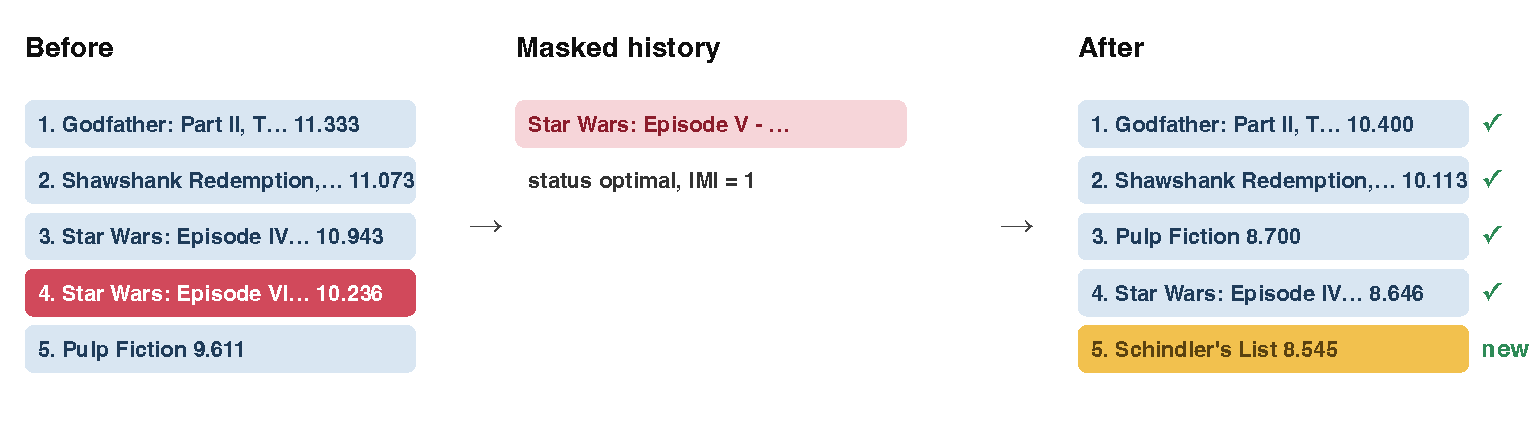
\includegraphics[width=\linewidth]{fig_worked.pdf}
\caption{Worked example, $K=5$. Left: the original list; the target is red. Centre: the masked history interaction. Right: the list after re-ranking. Blue rows are retained movies, the gold row is the replacement, and a tick marks a retained movie that keeps a qualifying path. Scores are the path-additive scores.}
\label{fig:worked}
\end{figure}



\section{Experimental setup}
\label{sec:setup}

\paragraph{Data.} MovieLens-1M~\cite{harper2015movielens} ratings of at least 4 are positives. Movies are linked to the
Microsoft Satori knowledge graph through the public RippleNet release~\cite{wang2018ripplenet}. Last.fm artist plays are
the HetRec 2011 release~\cite{cantador2011hetrec}, linked to Satori through the public KGCN release~\cite{wang2019kgcn};
every play count of at least 1 is a positive. We keep items with a knowledge-graph link, then a core of 10 users and 5
items on MovieLens and of 5 users and 3 items on Last.fm, and we drop entities shared by only one remaining item.
Relations with fewer than 200 links on MovieLens, or 20 on Last.fm, are dropped. This leaves \MLDataUsers{} users and
\MLDataItems{} movies on MovieLens, all of them still linked, and \LFDataUsers{} users and \LFDataItems{} artists on
Last.fm, of which \LFItemsKG{} keep a link after the relation filter. Each user's positives are shuffled and split
70/10/20 into train, validation and test. Co-occurrence, popularity and the path weights are fit on the training split
only. Validation chooses the baseline hyperparameters. Explanations are computed on the training history, which is the
input of the deployed model.

\paragraph{Backbone accuracy.} \Cref{tab:acc} reports Recall@20 and NDCG@20 on the test split, ranked with the same tie
rule as the solver. The backbone is competitive with item-based collaborative filtering and with BPR matrix
factorisation on both datasets, so the explanations concern a reasonable recommender rather than a toy one. The learned
weight on collaborative paths is $\theta_{\mathrm{co}}=\MLThetaCo$ on MovieLens and $\LFThetaCo$ on Last.fm. The
popularity weight is $\beta=\MLBeta$ on MovieLens and $\LFBeta$ on Last.fm. The knowledge-graph-only row is a
separately trained model with the collaborative relation removed.

\begin{table}[t]
\centering
\caption{Test-set top-20 accuracy (\%). MovieLens: \MLDataUsers{} users. Last.fm: \LFDataUsers{} users. ItemKNN uses
cosine similarity; validation selected the full neighbourhood over neighbourhood sizes all, 50 and 200. BPR-MF has 64
factors and stopped after 10 epochs on the validation split.}
\label{tab:acc}
\begin{tabular}{lcccc}
\toprule
 & \multicolumn{2}{c}{MovieLens-1M} & \multicolumn{2}{c}{Last.fm} \\
Model & Recall@20 & NDCG@20 & Recall@20 & NDCG@20 \\
\midrule
Popularity & \MLRecPop & \MLNdcgPop & \LFRecPop & \LFNdcgPop \\
ItemKNN & \MLRecItemKNN & \MLNdcgItemKNN & \LFRecItemKNN & \LFNdcgItemKNN \\
BPR-MF & \MLRecBPR & \MLNdcgBPR & \LFRecBPR & \LFNdcgBPR \\
Backbone, KG paths only & \MLRecKG & \MLNdcgKG & \LFRecKG & \LFNdcgKG \\
Backbone, KG and collaborative paths & \MLRecFull & \MLNdcgFull & \LFRecFull & \LFNdcgFull \\
\bottomrule
\end{tabular}
\end{table}

\paragraph{Protocol.} On each dataset we draw \UsersPerQ{} users from each quartile of training-history length
(\NUsers{} users, seed 1) and take every item of each user's top-10 list as a target, giving \NPairs{} pairs. The main
configuration is $K=10$, $\alpha=0.5$, $\phi=0$ and $\varepsilon=\Eps$. Three further MovieLens samples, 25 users per
quartile, vary one factor each: the evidence threshold $\alpha\in\{0.25,0.5,0.75,1\}$ under C1 + C2 + C3; the list
size $K\in\{5,10,20\}$; and the margin $\varepsilon\in\{10^{-8},10^{-6},10^{-4}\}$, with exhaustive search wherever
$|D_u(t)|\le\EnumMax$. These samples are not the main sample. The exact solver has a budget of \TimeLimit{} seconds.
Certification uses \CertLimit{} seconds per re-solve.

\paragraph{Statistics.} Mask-size costs are paired. A difference is computed only on the pairs that are optimal in both
compared settings, because the hardest pairs drop out as constraints tighten. Each table states how many pairs and
users lie behind a difference. All 95\% intervals are percentile bootstrap intervals (\NBoot{} replicates) that
resample users within each history quartile and keep every target of a resampled user together.

\section{Results}
\label{sec:results}

\subsection{How often is surgical removal possible?}

\begin{table}[t]
\centering
\caption{Certified solver outcomes (\%). Each row is \NPairs{} pairs from \NUsers{} users, $K=10$, $\alpha=0.5$,
$\varepsilon=\Eps$. A mask exists when the outcome is optimal or feasible. The feasible share on MovieLens includes
the \MLCertUndecided{} claimed optima that the second HiGHS configuration did not confirm. The interval resamples users.}
\label{tab:status}
\resizebox{\linewidth}{!}{\begin{tabular}{llrrrrr}
\toprule
Dataset & Setting & Optimal & Feasible & Infeasible & Timeout & Exists [95\% CI] \\
\midrule
MovieLens-1M & C1 & 95.30 & 4.70 & 0.00 & 0.00 & 100.00 [100.00, 100.00] \\
MovieLens-1M & C1 + C3 & 83.85 & 0.75 & 15.40 & 0.00 & 84.60 [82.29, 86.74] \\
MovieLens-1M & C1 + C2 & 80.35 & 2.95 & 16.55 & 0.15 & 83.30 [80.92, 85.75] \\
MovieLens-1M & C1 + C2 + C3 & 71.20 & 1.90 & 26.90 & 0.00 & 73.10 [70.11, 76.05] \\
Last.fm & C1 & 95.70 & 0.00 & 4.30 & 0.00 & 95.70 [94.75, 96.60] \\
Last.fm & C1 + C3 & 82.85 & 0.00 & 17.15 & 0.00 & 82.85 [80.80, 84.75] \\
Last.fm & C1 + C2 & 30.05 & 0.00 & 69.95 & 0.00 & 30.05 [28.05, 31.90] \\
Last.fm & C1 + C2 + C3 & 28.05 & 0.00 & 71.95 & 0.00 & 28.05 [26.15, 30.00] \\
\bottomrule
\end{tabular}
}
\end{table}

\Cref{tab:status} is the outcome of every main-sample pair after the second HiGHS configuration. On MovieLens, removing the target alone is
always possible: a mask exists for \MLAExists\% of pairs (\MLAOpt\% with a confirmed minimum, \MLAFeas\% with a
verified mask whose minimality was not confirmed). Keeping the other nine items lowers this to \MLBExists\%
[\MLBExistsLo, \MLBExistsHi], and keeping their evidence as well lowers it to \MLCExists\% [\MLCExistsLo,
\MLCExistsHi]. The pairs without a mask are proven infeasible (\MLBInf\% under C1 + C2, \MLCInf\% under
C1 + C2 + C3) except for \MLBTout\% of pairs under C1 + C2, which reached neither a mask nor a proof. On Last.fm,
removal itself fails for \LFAInf\% of pairs. Keeping the list is the binding constraint: existence falls to
\LFBExists\% [\LFBExistsLo, \LFBExistsHi], and requiring the evidence as well leaves \LFCExists\% [\LFCExistsLo,
\LFCExistsHi]. Requiring the evidence without the list constraint, C1 + C3, leaves existence at \MLAThreeExists\% on
MovieLens and \LFAThreeExists\% on Last.fm, so the evidence constraint is affordable once the target is removed and the
list constraint is not. No main-sample pair has a retained item with an empty evidence set. No solve was killed.
Median solve times are \MLATime, \MLBTime{} and \MLCTime{} seconds for the three MovieLens settings; the longest
MovieLens solve took \MLATimeMax{} seconds.

Of the Last.fm pairs with no C1 + C2 + C3 mask, \LFCauseList\% are already impossible under C1 + C2. On MovieLens
that share is \MLCauseList\%; evidence entanglement accounts for \MLCauseEv\% and a joint conflict, in which
C1 + C2 and C1 + C3 are each feasible but not together, for \MLCauseJoint\%. On Last.fm those two causes are
\LFCauseEv\% and \LFCauseJoint\%.

\begin{table}[t]
\centering
\caption{Paired cost of a constraint: difference in minimum mask size, on the pairs that are optimal in both
settings. The interval resamples users.}
\label{tab:paired}
\resizebox{\linewidth}{!}{\begin{tabular}{llrrrr}
\toprule
Dataset & Comparison & Pairs (users) & Mean [95\% CI] & Median & Share $>0$ \\
\midrule
MovieLens-1M & C1+C2 $-$ C1 & 1535 (198) & 1.348 [1.185, 1.524] & 0 & 33.7\% \\
MovieLens-1M & C1+C2+C3 $-$ C1+C2 & 1401 (198) & 0.313 [0.250, 0.377] & 0 & 15.1\% \\
MovieLens-1M & C1+C3 $-$ C1 & 1598 (200) & 0.397 [0.325, 0.479] & 0 & 18.9\% \\
Last.fm & C1+C2 $-$ C1 & 601 (182) & 0.271 [0.212, 0.334] & 0 & 20.0\% \\
Last.fm & C1+C2+C3 $-$ C1+C2 & 561 (176) & 0.007 [0.002, 0.014] & 0 & 0.7\% \\
Last.fm & C1+C3 $-$ C1 & 1657 (200) & 0.020 [0.012, 0.029] & 0 & 1.8\% \\
\bottomrule
\end{tabular}
}
\end{table}

\Cref{tab:paired} is the cost on the pairs where both minima are confirmed. On MovieLens, keeping the list costs
\MLBAMean{} [\MLBALo, \MLBAHi] extra interactions on average (\MLBAN{} pairs, \MLBAUsers{} users), and keeping the
evidence costs another \MLCBMean{} [\MLCBLo, \MLCBHi] (\MLCBN{} pairs). Both medians are 0, and only \MLBAPos\% and
\MLCBPos\% of the pairs need any extra interaction, so the averages are carried by a minority of entangled pairs. On
Last.fm the same two costs are \LFBAMean{} [\LFBALo, \LFBAHi] and \LFCBMean{} [\LFCBLo, \LFCBHi]. The evidence cost
is positive but tiny: once a list-preserving mask exists, one more interaction is rarely required. No pair needs a
smaller mask under a stricter setting. Under the minimum masks the retained items reorder only moderately. Mean
Kendall's $\tau$ between their original and new order is \MLKendallB{} and \MLKendallC{} on MovieLens and
\LFKendallB{} and \LFKendallC{} on Last.fm.

\begin{figure}[t]
\centering
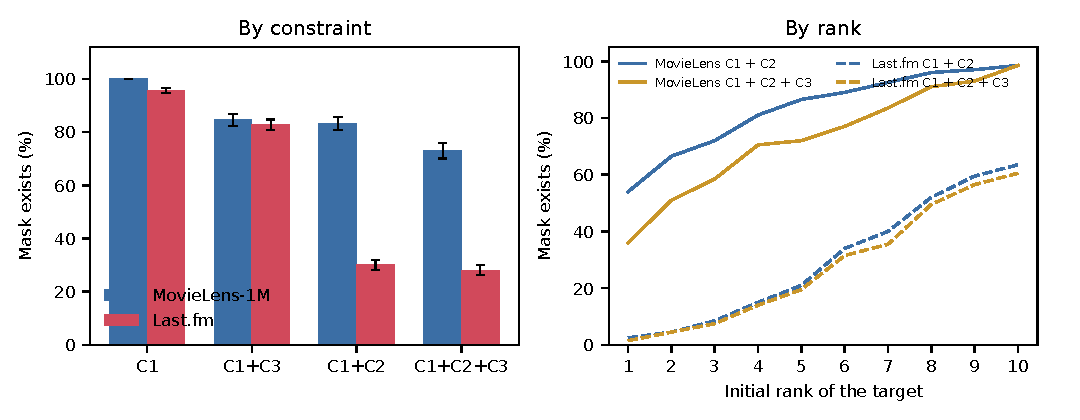
\includegraphics[width=\linewidth]{figures/feasibility.pdf}
\caption{Mask existence after the second HiGHS configuration. Left: by constraint, with the 95\% user-level bootstrap interval. Right:
by the target's initial rank, for C1 + C2 (blue) and C1 + C2 + C3 (gold); solid lines are MovieLens-1M and dashed
lines are Last.fm. Each point is 200 pairs.}
\label{fig:feas}
\end{figure}

\begin{table}[t]
\centering
\caption{Mask existence (\%) by the target's initial rank. Each cell is 200 pairs.}
\label{tab:rank}
\begin{tabular}{rcccc}
\toprule
Rank & ML C1+C2 & ML C1+C2+C3 & LF C1+C2 & LF C1+C2+C3 \\
\midrule
1 & 54.0 & 36.0 & 2.5 & 1.5 \\
2 & 66.5 & 51.0 & 4.5 & 4.5 \\
3 & 72.0 & 58.5 & 8.5 & 7.5 \\
4 & 81.0 & 70.5 & 15.0 & 14.0 \\
5 & 86.5 & 72.0 & 21.0 & 19.5 \\
6 & 89.0 & 77.0 & 34.0 & 31.5 \\
7 & 92.5 & 83.5 & 40.0 & 35.5 \\
8 & 96.0 & 91.0 & 52.0 & 49.5 \\
9 & 97.0 & 93.0 & 59.5 & 56.5 \\
10 & 98.5 & 98.5 & 63.5 & 60.5 \\
\bottomrule
\end{tabular}

\end{table}

\begin{table}[t]
\centering
\caption{Mask existence (\%) by training-history quartile, shortest to longest. Each cell is 500 pairs.}
\label{tab:quartile}
\begin{tabular}{lcccc}
\toprule
History quartile & ML C1+C2 & ML C1+C2+C3 & LF C1+C2 & LF C1+C2+C3 \\
\midrule
shortest & 57.2 & 42.8 & 11.8 & 9.4 \\
second & 82.6 & 66.4 & 27.2 & 24.8 \\
third & 93.8 & 86.8 & 36.0 & 34.4 \\
longest & 99.6 & 96.4 & 45.2 & 43.6 \\
\bottomrule
\end{tabular}

\end{table}

\paragraph{Rank matters most.} \Cref{fig:feas} and \Cref{tab:rank} show the same rank effect on both datasets.
A list-preserving mask exists for \MLBROne\% of MovieLens rank-1 targets and for \MLBRTen\% of rank-10 targets
(C1 + C2 + C3: \MLCROne\% and \MLCRTen\%). On Last.fm the rank-1 rates are \LFBROne\% and \LFCROne\%, against
\LFBRTen\% and \LFCRTen\% at rank 10. A borderline recommendation can usually be removed without side effects. The
strongest recommendation usually cannot, and on Last.fm it almost never can.

\paragraph{Short histories are more entangled.} \Cref{tab:quartile} stratifies by history length. The shortest
quartile has the lowest existence under C1 + C2 and under C1 + C2 + C3: \MLBQShort\% and \MLCQShort\% on MovieLens, against
\MLBQLong\% and \MLCQLong\% in the longest quartile, and \LFBQShort\% and \LFCQShort\% against \LFBQLong\% and \LFCQLong\% on Last.fm.
With few interactions, each one supports a large part of the list.

\subsection{Original problem versus margin variant}
\label{sec:semantics}

\begin{table}[t]
\centering
\caption{$P$ versus $\Peps$ on the MovieLens margin sample, for every pair with $|D_u(t)|\le\EnumMax$. Both problems
are solved by exhaustive search. The agreement column sums the three settings, so the denominator is three times the
number of pairs. The main samples were not enumerated.}
\label{tab:semantics}
\begin{tabular}{lccc}
\toprule
$\varepsilon$ & Pairs (users) & Status or optimum differs & MILP agrees \\
\midrule
$10^{-8}$ & 190 (19) & 0 & 570/570 \\
$10^{-6}$ & 190 (19) & 0 & 570/570 \\
$10^{-4}$ & 190 (19) & 0 & 570/570 \\
\bottomrule
\end{tabular}

\end{table}

\Cref{tab:semantics} compares $P$ with $\Peps$ at three margins. The enumerable pairs are \EnumPairs{} pairs from
\EnumUsers{} of the 100 sampled users. Feasibility and the optimum never differ, and the MILP agrees with the
$\Peps$ enumeration on every decided pair--setting combination. The two problems can differ when a mask needs a gap
smaller than $\varepsilon$ or an exact tie. On this sample, at these margins, they did not. On the pairs that are
too large to enumerate, the indirect check is the one in \Cref{tab:heuristics}: across every stored comparison of an
approximate method with the reported optimum, \SmallerThanOpt{} masks were smaller than that optimum and
\SuccessOnInf{} approximate masks succeeded on a pair the MILP had proved infeasible.

\subsection{Do constraint-unaware edits preserve the list?}

\begin{table}[t]
\centering
\caption{Approximate methods under C1 + C2 + C3. Success is the share of all \NPairs{} pairs for which the verifier
accepts the mask. Exact size is the share of those accepted masks, among pairs with a reported optimum, that have
that optimum's size. For the stop-at-C1 row, success is the share of pairs whose removal-only mask happens to
satisfy C1 + C2 + C3.}
\label{tab:heuristics}
\resizebox{\linewidth}{!}{\begin{tabular}{lcccc}
\toprule
 & \multicolumn{2}{c}{MovieLens-1M} & \multicolumn{2}{c}{Last.fm} \\
Method & success & exact size & success & exact size \\
\midrule
beam search & 63.45 & 95.90 & 28.05 & 100.00 \\
violation greedy & 62.05 & 90.72 & 27.15 & 98.89 \\
continuous, sigmoid & 71.30 & 68.52 & 26.60 & 97.18 \\
continuous, Gumbel & 71.35 & 63.50 & 26.30 & 95.25 \\
ranking-margin order & 45.40 & 75.96 & 14.35 & 91.64 \\
list-aware order & 44.20 & 72.18 & 18.75 & 93.33 \\
target-score order & 32.10 & 63.56 & 12.85 & 95.72 \\
target-score, stop at C1 & 21.80 & 76.17 & 11.75 & 97.45 \\
popularity order & 15.10 & 37.25 & 6.45 & 75.97 \\
random order & 15.10 & 26.49 & 8.15 & 77.30 \\
\bottomrule
\end{tabular}
}
\end{table}

The target-score order that stops at removal reaches C1 for \MLCStopCOne\% of MovieLens pairs and \LFCStopCOne\% of
Last.fm pairs. Among those edits, \MLCStopList\% and \LFCStopList\% keep the other nine items, and \MLCStopAll\% and
\LFCStopAll\% keep the items and their evidence. Stability is not a by-product of a minimal removal: it has to be
asked for. When the same orders are required to satisfy the constraints, beam search and the violation greedy come
closest to the exact solver. Beam search returns a verified mask on \MLCbeamSucc\% of MovieLens pairs and on
\LFCbeamSucc\% of Last.fm pairs, which is every Last.fm pair for which a mask exists, and the mask has the reported
size for \MLCbeamExact\% and \LFCbeamExact\% of its successes on proven optima. The violation greedy is close
(\MLCgreedyviolationSucc\% and \LFCgreedyviolationSucc\% success). The repaired continuous masks succeed more often
than beam search on MovieLens and less often at the exact size (\Cref{tab:heuristics}). Popularity and random orders
rarely satisfy the constraints. No approximate mask in the stored comparisons is smaller than a reported optimum
(\SmallerThanOpt{}), and none succeeds on a pair proved infeasible (\SuccessOnInf{}).

\subsection{Sensitivity}

\begin{table}[t]
\centering
\caption{Evidence threshold $\alpha$ on a separate MovieLens sample (100 users, 1{,}000 pairs, C1 + C2 + C3,
$K=10$). Outcomes are percentages. The mean size is over the pairs whose optimum was confirmed, so pairs that
become infeasible drop out of it.}
\label{tab:alpha}
\begin{tabular}{ccccc}
\toprule
$\alpha$ & Exists & Optimal & Infeasible & Mean $|M|$ on optima \\
\midrule
0.25 & 79.8 & 76.0 & 20.2 & 7.19 \\
0.50 & 76.2 & 73.0 & 23.8 & 6.99 \\
0.75 & 72.9 & 70.8 & 27.1 & 6.99 \\
1.00 & 69.9 & 68.3 & 30.1 & 6.92 \\
\bottomrule
\end{tabular}

\end{table}

\begin{table}[t]
\centering
\caption{List size $K$ on a separate MovieLens sample (100 users, every top-$K$ item). Outcomes are percentages.
The $K=10$ row is not the main sample.}
\label{tab:K}
\begin{tabular}{ccccccc}
\toprule
 & \multicolumn{2}{c}{C1} & \multicolumn{2}{c}{C1 + C2} & \multicolumn{2}{c}{C1 + C2 + C3} \\
$K$ & exists & timeout & exists & timeout & exists & timeout \\
\midrule
5 & 100.00 & 0.00 & 93.20 & 0.00 & 88.00 & 0.00 \\
10 & 100.00 & 0.00 & 84.70 & 0.20 & 74.90 & 0.10 \\
20 & 100.00 & 0.00 & 70.95 & 1.75 & 54.70 & 0.00 \\
\bottomrule
\end{tabular}

\end{table}

\Cref{tab:alpha} raises the evidence threshold. Mask existence under C1 + C2 + C3 falls from \AlphaExistsLow\% at
$\alpha=0.25$ to \AlphaExistsOne\% at $\alpha=1$. The mean size on the pairs that remain optimal does not grow,
because the pairs that become infeasible leave the average. \Cref{tab:K} varies the list. A list-preserving mask
exists for \KFiveBExists\% of pairs at $K=5$ and \KTwentyBExists\% at $K=20$ (C1 + C2 + C3: \KFiveCExists\% and
\KTwentyCExists\%). Removal alone is solved for every pair at every $K$. At $K=20$, \KTwentyBTout\% of the C1 + C2 pairs
time out. Longer lists are harder to preserve because more items share the target's support.

\section{Discussion and limitations}

\paragraph{What the numbers mean.} On MovieLens, most recommendations, and almost all borderline ones, have a small
edit that removes the item and leaves the rest of the list and its evidence intact. The strongest recommendations,
and the users with the shortest histories, often do not. On Last.fm the list constraint binds much earlier: a
list-preserving edit exists for about a third of pairs, and for the top-ranked item almost never. In both datasets
the failures are mostly proved, not merely unsolved. The exact formulation turns that entanglement into a measured
quantity. One MovieLens optimum of size 4 was replaced by a verified optimum of size 3, and \MLCertUndecided{}
claimed MovieLens optima remain feasible rather than optimal because a second configuration of HiGHS did not
confirm them. That cross-check is not a certificate.

\paragraph{Why Last.fm is harder.} Full-constraint existence is \MLCExists\% on MovieLens and \LFCExists\% on
Last.fm. The drop is already present under C1 + C2: \MLBExists\% against \LFBExists\%. Adding C3 changes Last.fm
only from \LFBExists\% to \LFCExists\%. On the Last.fm pairs where C1 + C2 + C3 is infeasible, the recorded cause
is list entanglement for \LFCauseList\% of those pairs. Evidence entanglement accounts for \LFCauseEv\% and a joint conflict for \LFCauseJoint\%.
Two stored differences travel with this gap, and this paper does not separate them experimentally. The learned
popularity weight is $\beta=\MLBeta$ on MovieLens and $\beta=\LFBeta$ on Last.fm; the weights were fit separately,
so this is not a controlled ablation with the other weights held fixed. The permitted mask domain $D_u(t)$ covers
\MLScope\% of training-history interactions on the MovieLens main pairs and \LFScope\% on Last.fm. No main-sample
pair on either dataset has an empty evidence set (\MLEvFree{} and \LFEvFree{}). A retrained popularity ablation,
and a run that expands the mask domain to the whole history, were not done. The association is that Last.fm fails
the list constraint, not that its evidence paths are uniquely entangled.

\paragraph{Limitations.} (i) The backbone is additive by design, so that path contributions are exact and C3 can be
checked in closed form. Non-additive recommenders need a single-path-disabling definition of contribution and an
approximate solver; this is study~2. (ii) The exact solver works on $\Peps$ with $M\subseteq D_u(t)$. Agreement with
$P$ was checked by enumeration on the \EnumPairs{} enumerable pairs of the margin sample, from \EnumUsers{} users,
mostly short histories. That is not a general equivalence. Infeasibility for $\Peps$, or outside $D_u(t)$, is not
infeasibility for $P$ on the whole history. (iii) The sensitivity samples have 100 users and are separate from the
main 200. (iv) The heuristics, the beam and the continuous masks are our own procedures on this backbone. They are
not GREASE, LXR, ACCENT, PRINCE, TRACE or the counterfactual support-set method of Zhang et al. Those methods were
not run. The blocker is concrete. GREASE trains a surrogate GNN and perturbs its adjacency; ACCENT uses influence
functions on a different model; LXR trains an explainer network; PRINCE explains personalised PageRank; Zhang et al.\
learn a retention mask for a frozen LightGCN. None of their official implementations is a solver for $P_\varepsilon$
on this path-additive backbone, and adapting them would be a new experiment. No number in this paper is such an
experiment. Zhang et al.\ is cited from the authors' preprint; the venue and DOI were not confirmable from the
publisher, and the acronym CoSRec also names an unrelated SIGIR 2025 dataset, so the paper is cited by title.
(v) The knowledge graphs are the Satori linkages
released with RippleNet and KGCN, not KB4Rec or Freebase. Entity names are not in the rehashed release.
(vi) The literature check was focused rather than
systematic. We do not claim to be the first method of this kind.
(vii) The backbone is static. User preferences drift over
time~\cite{tahmasbi2018temporal,tahmasbi2021coupled}; with time-dependent scores the score row of an interaction would
change between requests, and extending evidence-preserving counterfactuals to such dynamic recommenders is future
work.

\section{Conclusion}

EPIC-Rec asks for counterfactual explanations that remove one recommendation without collateral damage to the rest
of the list or to its evidence. On this additive path recommender the margin problem on $D_u(t)$ has a
mixed-integer formulation, and returned masks are re-ranked independently. On
MovieLens a feasible mask is usual, except for the items the user is most strongly recommended. On Last.fm,
keeping the rest of the list is possible for only a minority of recommendations. The formulation gives a test bed
for explainers that claim list-level faithfulness. It does not by itself establish that claim for other backbones.

\paragraph{Code and data availability.} The implementation is at
\url{https://github.com/MehrdadJalali-AI/EPIC-Rec}. The commit that contains this revision is recorded in
\texttt{manuscript/REVISION}. Aggregated tables in \texttt{results/report/tables} and the compact per-instance
exact statuses in \texttt{results/published} are the machine-readable results behind the tables and
\Cref{fig:charts}. \texttt{scripts/manuscript\_from\_report.py} writes \texttt{numbers.tex} and the result tables
from those aggregates. \texttt{scripts/fig1\_from\_results.py} draws the charts in \Cref{fig:overview} from the same
files. The worked example is regenerated by \texttt{scripts/export\_worked\_example.py}. The prose is not generated
automatically. The full \texttt{records.jsonl} files are produced by the runner and are not stored in git because
each main file is about 80\,MB; the commands that regenerate them are in \texttt{docs/reproducibility.md}. Raw
datasets and credentials are not redistributed. HiGHS is used through \texttt{highspy} 1.15.1.

\bibliographystyle{plainnat}
\bibliography{refs}
\end{document}
